\documentclass{beamer}
\usetheme{Boadilla}
%\usetheme{polimi}

\usefonttheme{professionalfonts}
%\usefonttheme{serif}

\usepackage[utf8]{inputenc}
\usepackage[italian]{babel}
\usepackage{fancyhdr}
\usepackage{graphicx}
\usepackage{amssymb}
\usepackage{amsthm}
\usepackage[parfill]{parskip}
\usepackage{mathtools}
\usepackage{tikz}
\usetikzlibrary{decorations.pathreplacing,calc}
\usepackage{bigints}
\usepackage[scr=boondox]{mathalfa}
\usepackage{centernot}
\usepackage{ifthen}
\usepackage{xfrac}
\usepackage{nicefrac}
\usepackage{makecell}
\usepackage[makeroom]{cancel}
\usepackage{bm}

\usepackage{multirow}
\usepackage{cancel}
\usepackage{textpos}
\usepackage{color}
\usepackage{subcaption}
\usepackage[percent]{overpic}
\usepackage{pdfpages}

% Delimiters
\DeclarePairedDelimiter\abs{\lvert}{\rvert}
\DeclarePairedDelimiter\norm{\lVert}{\rVert}

% Utilities
\newcommand{\Fixvmode}{\leavevmode\vspace{-\baselineskip}}
\newcommand{\tikzmark}[2]{\tikz[remember picture,baseline=(#1.base)]{\node[inner sep=0pt] (#1) {#2};}}

% Symbols
\newcommand{\indep}{\mathrel{\text{\scalebox{1.07}{$\perp\mkern-10mu\perp$}}}}

% Bold letters for vectors
\newcommand{\kk}{\boldsymbol K}
\newcommand{\uu}{\boldsymbol u}
\newcommand{\yy}{\boldsymbol y}

% Calligraphic letters
\newcommand{\Ac}{\mathcal A}
\newcommand{\Bc}{\mathcal B}
\newcommand{\Cc}{\mathcal C}
\newcommand{\Dc}{\mathcal D}
\newcommand{\Ec}{\mathcal E}
\newcommand{\Fc}{\mathcal F}
\newcommand{\Gc}{\mathcal G}
\newcommand{\Hc}{\mathcal H}
\newcommand{\Ic}{\mathcal I}
\newcommand{\Jc}{\mathcal J}
\newcommand{\Kc}{\mathcal K}
\newcommand{\Lc}{\mathcal L}
\newcommand{\Mc}{\mathcal M}
\newcommand{\Nc}{\mathcal N}
\newcommand{\Oc}{\mathcal O}
\newcommand{\Pc}{\mathcal P}
\newcommand{\Qc}{\mathcal Q}
\newcommand{\Rc}{\mathcal R}
\newcommand{\Sc}{\mathcal S}
\newcommand{\Tc}{\mathcal T}
\newcommand{\Uc}{\mathcal U}
\newcommand{\Vc}{\mathcal V}
\newcommand{\Wc}{\mathcal W}
\newcommand{\Xc}{\mathcal X}
\newcommand{\Yc}{\mathcal Y}
\newcommand{\Zc}{\mathcal Z}

% Double pipe letters
\newcommand{\QQ}{\mathbb Q}
\newcommand{\RR}{\mathbb R}
\newcommand{\ZZ}{\mathbb Z}

%% \bigcdot a dot for arguments in functions
\makeatletter
\newcommand*\bigcdot{\mathpalette\bigcdot@{.5}}
\newcommand*\bigcdot@[2]{\mathbin{\vcenter{\hbox{\scalebox{#2}{$\m@th#1\bullet$}}}}}
\makeatother

% Arrows
\newcommand{\RArr}[1]{\parbox{#1}{\tikz{\draw[->](0,0)--(#1,0);}}}
\newcommand{\LArr}[1]{\parbox{#1}{\tikz{\draw[<-](0,0)--(#1,0);}}}
\newcommand{\UArr}[1]{\parbox{#1}{\tikz{\draw[->](0,0)--(0,#1);}}}
\newcommand{\DArr}[1]{\parbox{#1}{\tikz{\draw[<-](0,0)--(0,#1);}}}
\newcommand{\VArr}[1]{\parbox{#1}{\tikz{\draw[-](0,0)--(0,#1);}}}


\title[Numerical solvers for ODEs]{\textbf{Adaptive numerical solvers}}
\subtitle{for Ordinary Differential Equations}
\author[Guindani, Vidulis]{Bruno Guindani \\ Michele Vidulis}
\institute[PoliMi]{
\includegraphics[scale=.5]{etc/logo_long.jpg}}
\date[2019/07/22]{July 22, 2019}

\begin{document}

\frame{  %#01
	\titlepage
	{ \color{blue}
	\begin{center}
		\href{https://github.com/poliprojects/apc-project}
		{https://github.com/poliprojects/apc-project}
	\end{center}
	}
}

%\addtobeamertemplate{frametitle}{}{
%	\begin{textblock*}{100mm}(.85\textwidth,-0.5cm)
%		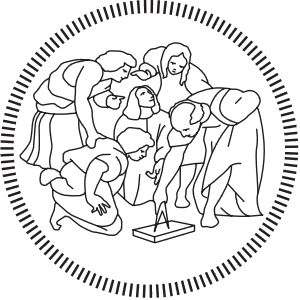
\includegraphics[scale=0.1]{etc/logo_only.png}
%	\end{textblock*}
%}

\begin{frame}[c] %#02
	\begin{center}
		\Huge \color{blue} Introduction
	\end{center}
\end{frame}


\begin{frame} %#03
	\frametitle{Ordinary differential equations (ODE)}
	Given $I = [t_0, t_F] \subset \RR, \ \ f(t,\yy): I \times \RR^n \to \RR^n,
	\quad f \in C^1$, and $t_0 \in I, \yy_0 \in \RR^n$:
	\begin{center}
		\textbf{Initial Value Problem (IVP)}: \\[15pt]
		find a $C^1$ function $\yy(t): I \to \RR^n$ that solves
		$$
		\begin{cases}
		\yy'(t) = f( t,\yy(t) ) \qquad \text{with } t \in I \\
		\yy(t_0) = \yy_0
		\end{cases}
		$$
		(first order ODE)
		%Ordinary: derive only wrt y
		%Higher-order EDOs can be reduced to a set of order 1 EDOs
	\end{center}
	\vspace{10pt}
	Existence and uniqueness guaranteed under \textit{Lipschitz continuity} of $f$
\end{frame}


\begin{frame} %#04
	\frametitle{Iterative methods} %TODO remove slide?
	\begin{itemize}
		\item Discretization of time into $N$ intervals: $t_0, \ t_1, \ \dots, \ t_{N} = t_F$ through a scretization step $h$: $t_{n+1} = t_n + h$, with $n = 0, 1, \dots, N$
		\item $\yy(t_n)$ is numerically approximated by $\uu_n$:
		\begin{center}
			$\uu_0 = \yy_0, \uu_1, \dots, \uu_{N} \in \RR^n$
			% iteratively updated
		\end{center}
		\pause
		\item In \textbf{single-step methods}, $\uu_{n+1}$ depends directly only on the one previous step $\uu_{n}$:
		$$ \uu_{n+1} = \uu_{n} + h \ \phi(t_n, \, h, \, \uu_n, \, \uu_{n+1}, \, f) $$
		\item In \textbf{explicit} methods, $\uu_{n+1}$ does not appear in $\phi$
		\item In \textbf{implicit} methods, $\uu_{n+1}$ appears in $\phi$
		\begin{center}
			\vspace{-5pt}
			$\implies$ nonlinear equations
		\end{center}
	\end{itemize}
\end{frame}


\begin{frame} %#05
	\frametitle{Runge-Kutta methods}
	\begin{itemize}
		\item Family of \textbf{single-step} methods
		\item Weighted average of $s$ evaluations (\textbf{stages}) of $f$: \\[-20pt]
		\begin{align*}
			\uu_{n+1} = \uu_{n} + h \sum_{i=1}^s b_i \kk_i \quad \text{with} \\[-5pt]
			\kk_i = f(t_0 + c_i h, \ \uu_n + \sum_{j=1}^s a_{ij} \kk_j)
		\end{align*}
		\pause
		\vspace{-22pt}
		\item \textit{Butcher tableau}:
		\begin{center}
			\begin{tabular}{c|ccc}
				$c_1$ & $a_{11}$ & $\dots$ & $a_{1s}$ \\
				\vdots & & $\ddots$ & \\
				$c_s$ & $a_{s1}$ & & $a_{ss}$ \\
				\hline
				& $b_1$ & $\dots$ & $b_s$
			\end{tabular}
		\hspace{30pt} with $c_i = \sum_j a_{ij}$
		\pause
		\end{center}
		\item $O(s n^2)$ if $f$ linear
		\item Explicit if $[a_{ij}]_{ij}$ is lower triangular
	\end{itemize}
\end{frame}


\begin{frame} %#06
	\frametitle{Examples of RK variants (1)}
	\begin{itemize}
		\item \textbf{Forward Euler} (FE) (explicit):
		$$ a = 0, \ b = 1, \ c = 0 $$
		$$ \uu_{n+1} = \uu_{n} + h f(t_n, \uu_n) $$
		\item RK4 (standard) (explicit): \\
		\begin{center}
			\begin{tabular}{c|cccc}
				$0$ & & & & \\
				$\frac 1 2$ & $\frac 1 2$ & & & \\
				$\frac 1 2$ & & $\frac 1 2$ & & \\
				$1$ & & & 1 & \\
				\hline
				& $\frac 1 6$ & $\frac 1 3$ & $\frac 1 3$ & $\frac 1 6$
				\end{tabular}
		\end{center}	
	\end{itemize}
\end{frame}


\begin{frame} %#07
	\frametitle{Examples of RK variants (2)}
	\begin{itemize}
		\item Heun (explicit):
		\begin{center}
			\begin{tabular}{c|cc}
				$0$ &     & \\
				$1$ & $1$ & \\
				\hline
				& $\frac 1 2$ & $\frac 1 2$
			\end{tabular}
		\end{center}
		\item \textbf{Iserles-Nørsett} (implicit):
		\begin{center}
			\begin{tabular}{c|cccc}
				$\frac{1}{3}$ & $\frac{1}{3}$ & & & \\
				$\frac{2}{3}$ & $\frac{1}{3}$ & $\frac{1}{3}$ & & \\
				$\frac{21+\sqrt{57}}{48}$ & & & $\frac{21+\sqrt{57}}{48}$ & \\
				$\frac{21-\sqrt{57}}{48}$ & & & $\frac{3-\sqrt{57}}{24}$ & $\frac{21+\sqrt{57}}{48}$ \\
				\hline
				& $\frac{9+3\sqrt{57}}{16}$ & $\frac{9+3\sqrt{57}}{16}$ & $-\frac{1+3\sqrt{57}}{16}$ & $-\frac{1+3\sqrt{57}}{16}$
				\end{tabular}
		\end{center}
	\end{itemize}
\end{frame}


\begin{frame} %#08
\frametitle{Convergence analysis for RK}
	\begin{itemize}
		\item \textbf{Convergence} $\to$ absolute error: $\norm{y_n - u_n} \simeq O(h^q)$
		\item \textbf{Consistence} $\to$ truncation error: $\max_n \norm{\tau_n(h)} \simeq O(h^q)$
		\item Under reasonable Lipschitz continuity assumptions on $\phi$, a single-step method which is consistent is also convergent
		\pause
		\item Runge-Kutta is consistent iff $\sum_i b_i = 1$ $\implies$ \textbf{convergent}
		\item Steep limitations on order of convergence:
		\begin{itemize}
			\item Maximum order is the number of stages
			\item If $s \ge 5$, equality cannot be achieved in explicit variants \\[15pt]
		\end{itemize}
	\end{itemize}
	\begin{center}
		\begin{tabular}{c|cccc}
			order & 5 & 6 & 7 & 8\\
			\hline
			minimum $s$ & 6 & 7 & 9 & 11 
		\end{tabular}
	\end{center}
	% Ex: Forward and backward Euler are order 1 methods
\end{frame}


\begin{frame} %#09
	\frametitle{Adaptive methods}
	\begin{itemize}
		\item Step $h$ is \textbf{updated} at every iteration adaptively, i.e. based on the trend of the solution
		\begin{itemize}
			\item Small $h$ near steep slopes, large $h$ near flat points
			% In model problem, lam(t) decreasing => function is flat
			\item \textit{A posteriori} \textbf{estimate of error} is needed
			\item Compute two-round solution with $\frac{h}{2}$, with single-round solution with $h$
		\end{itemize}
		\item No need for input of ``correct'' step
		\item Computational gain
	\end{itemize}
\end{frame}


\begin{frame} %#10
	\frametitle{Consistency of adaptive methods}
	Forward Euler:
	\begin{itemize}
		\item Truncation errors:
		$$ e_h = h^2/2 y''(\xi), \qquad e_{h/2} = h^2/8 y''(\eta) \cdot 2 + o(h^2) $$
		\item Error estimate:
		$$ \abs{u_{h/2} - u_h} \simeq \abs{e_{h/2}} \simeq h^2/4 \abs{y''(\widehat\eta)}
		+ o(h^2) \stackrel{\downarrow}{<} \frac{\varepsilon}{2}
		\quad \text{(tolerance)} $$
	\end{itemize}
	\pause
	Runge-Kutta:
	\begin{itemize}
		\item \dots %TODO!!! (RK consistency)
	\end{itemize}
\end{frame}


\begin{frame}[c] %#11
\begin{center}
	\Huge \color{blue} Code structure
\end{center}
\end{frame}


\begin{frame} %#12
	\frametitle{Code structure}
	\begin{center}
		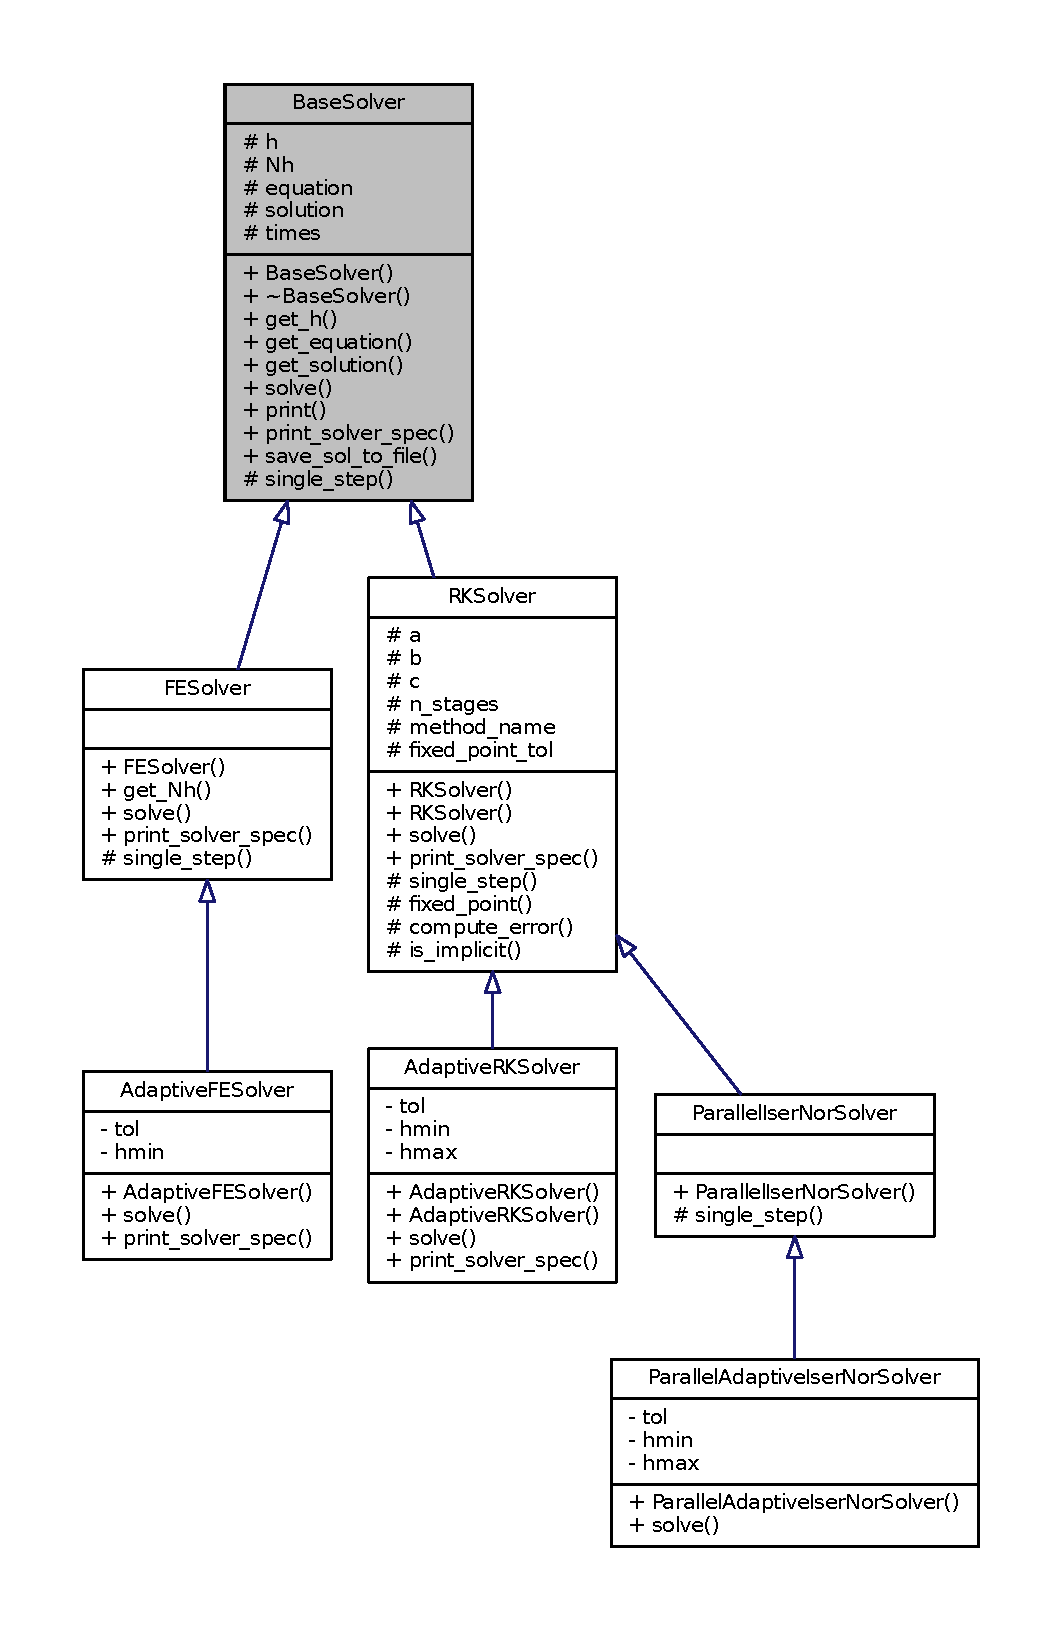
\includegraphics[width=0.45 \linewidth]{etc/classes_full.pdf}
	\end{center}
\end{frame}


\begin{frame} %#13
	\frametitle{Base classes}
	\begin{figure}
		\begin{subfigure}{.5\textwidth}
			\begin{center}
				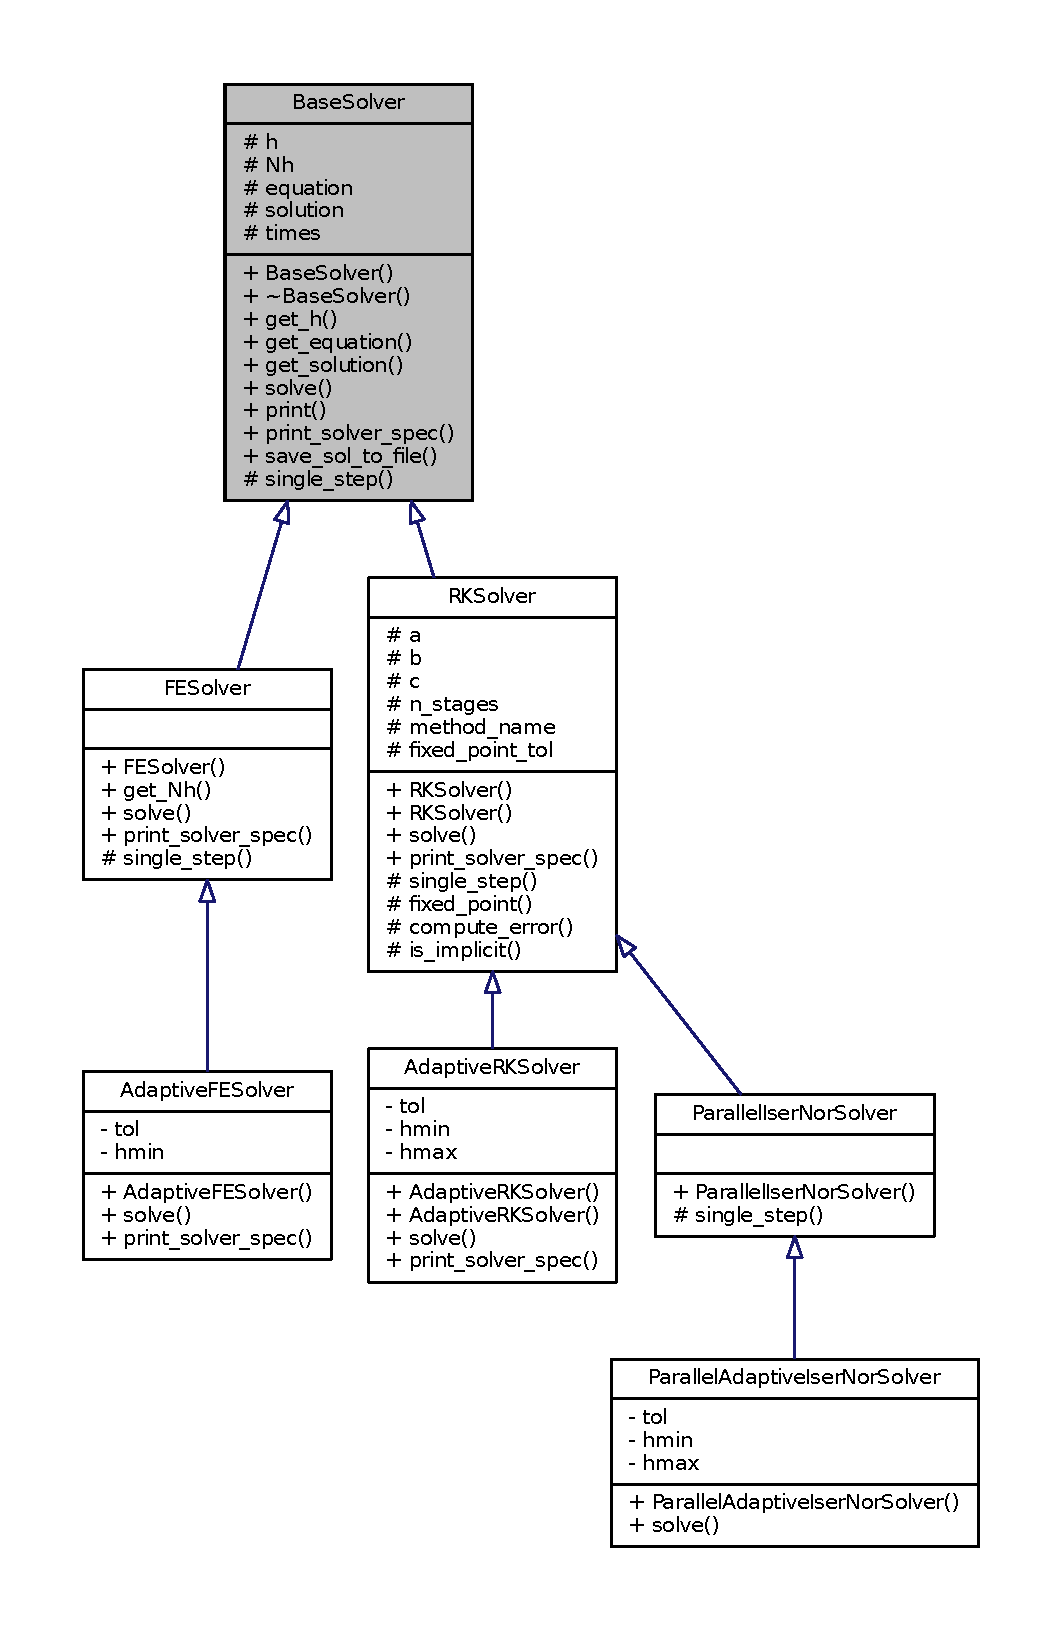
\includegraphics[width=0.5 \linewidth]{etc/classes_full.pdf} %base
			\end{center}
		\end{subfigure}%
		\begin{subfigure}{.5\textwidth}
			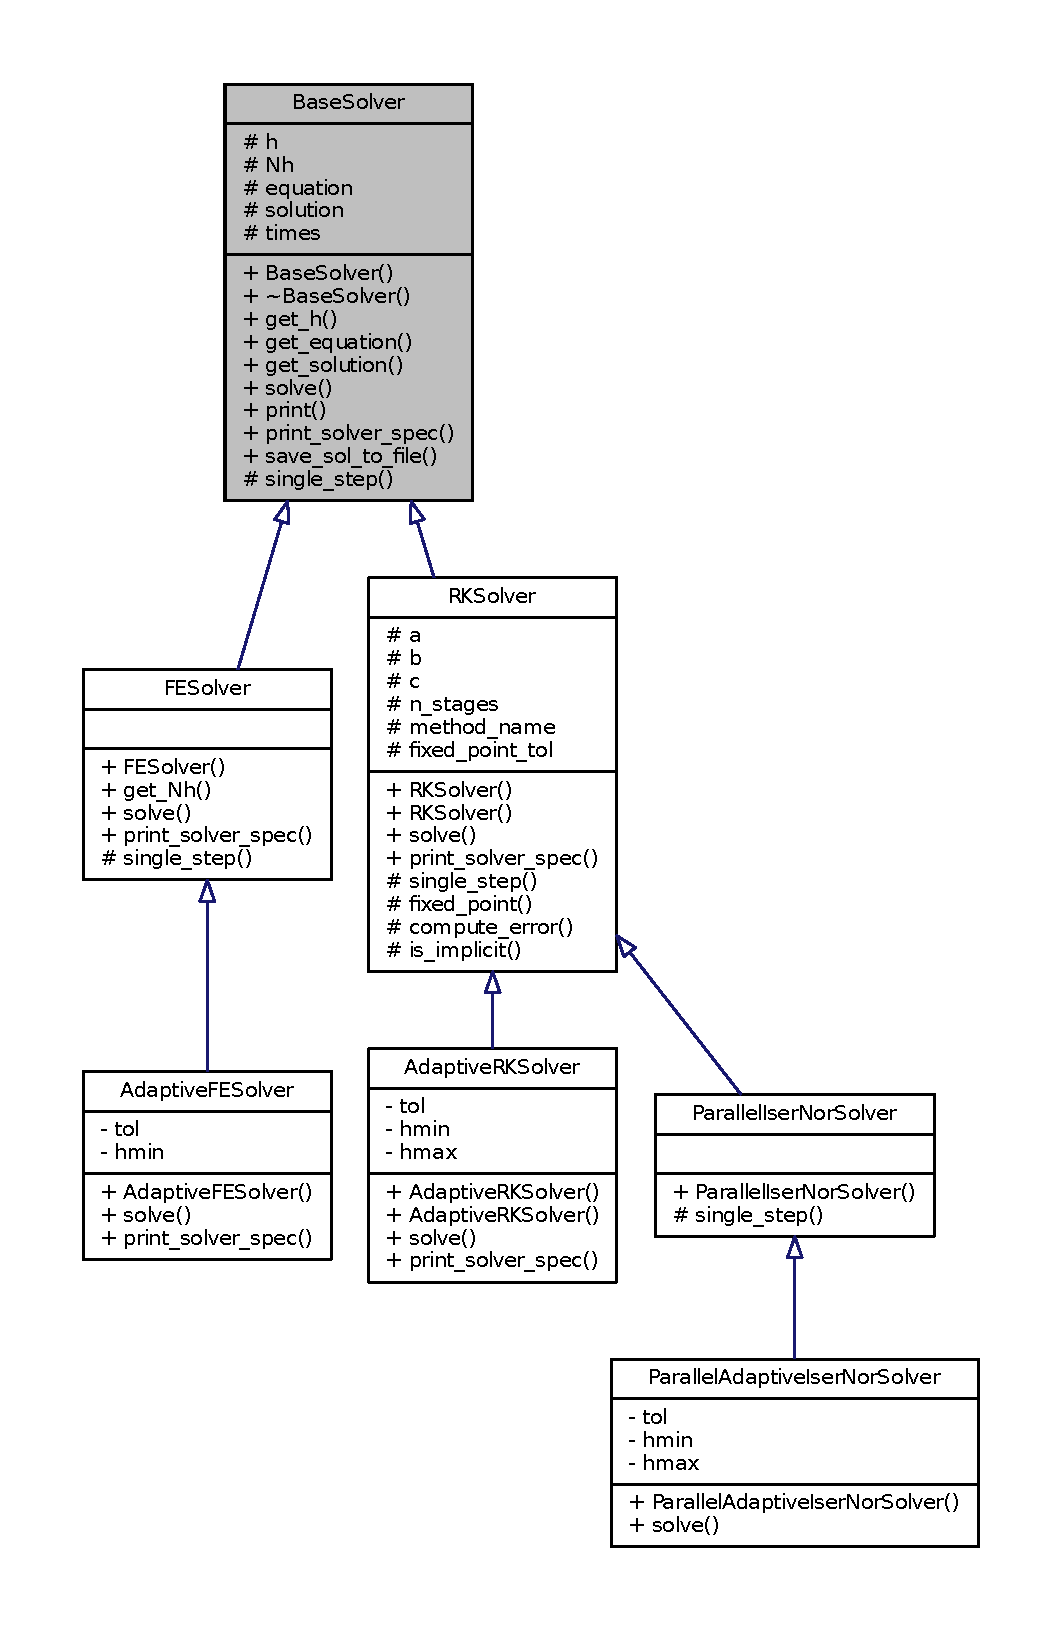
\includegraphics[width=\linewidth]{etc/classes_full.pdf} %plain
		\end{subfigure}
	\end{figure}
\end{frame}


\begin{frame} %#14
	\frametitle{Adaptive classes}
	\centering
	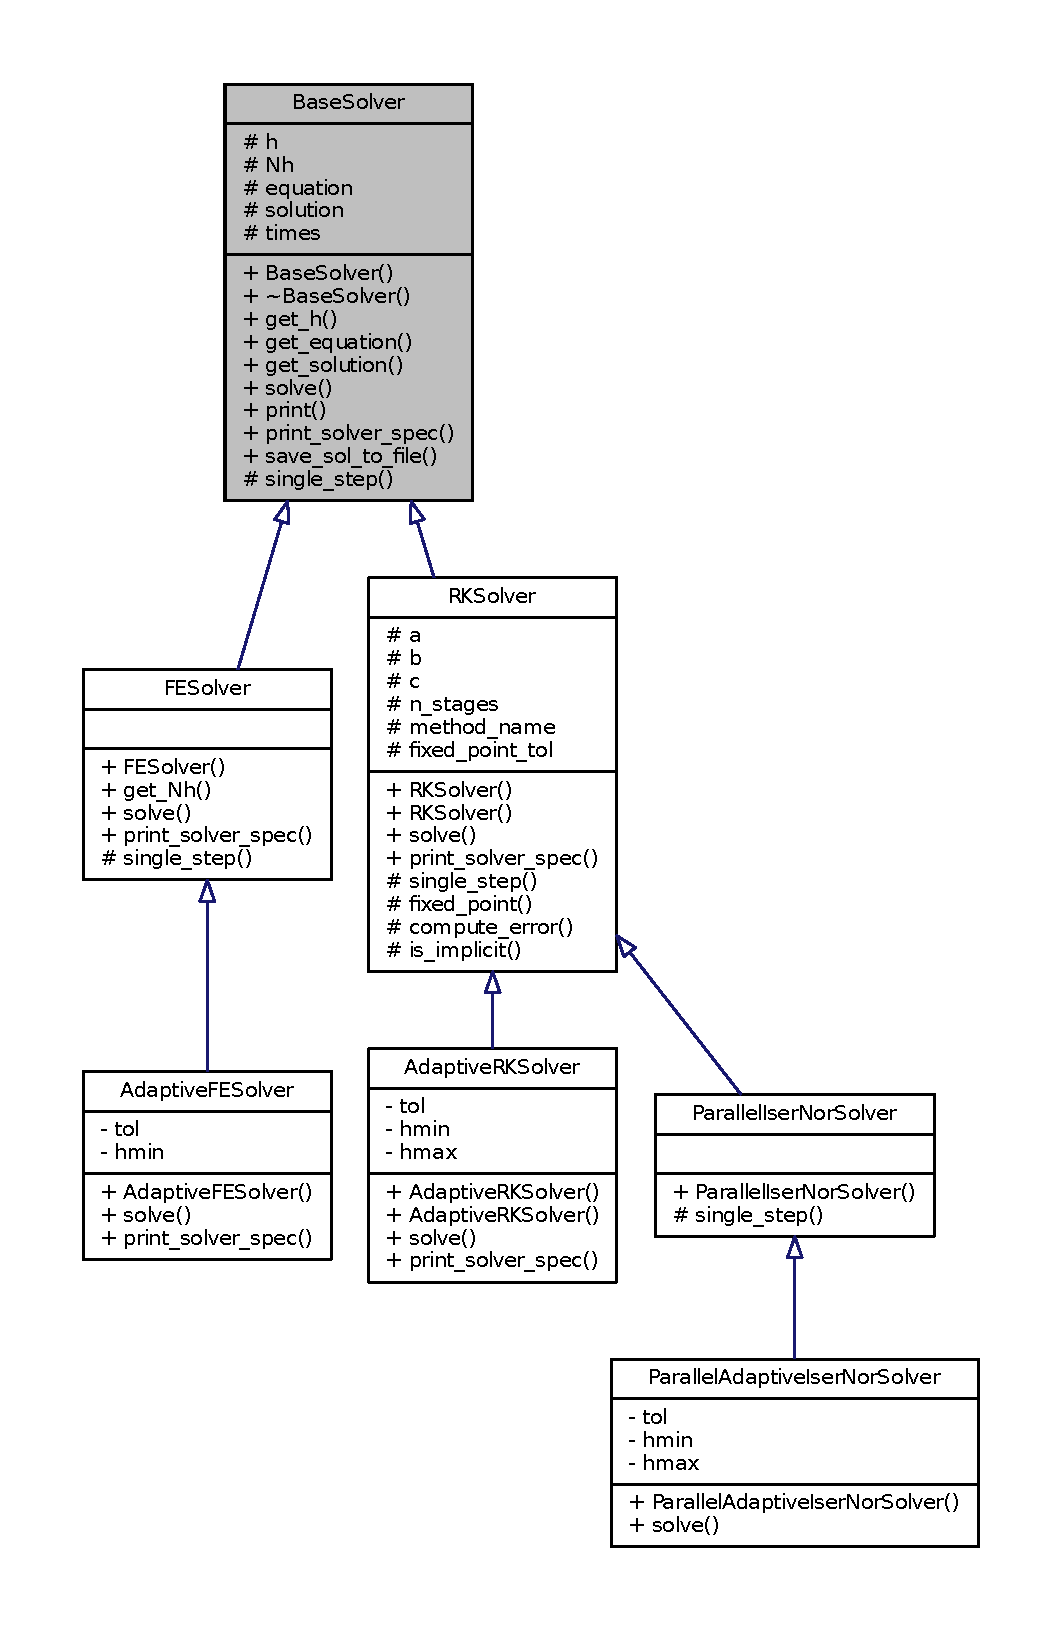
\includegraphics[width=\linewidth]{etc/classes_full.pdf} %adaptive
\end{frame}


\begin{frame} %#15
	\frametitle{Dependencies}
	\centering
	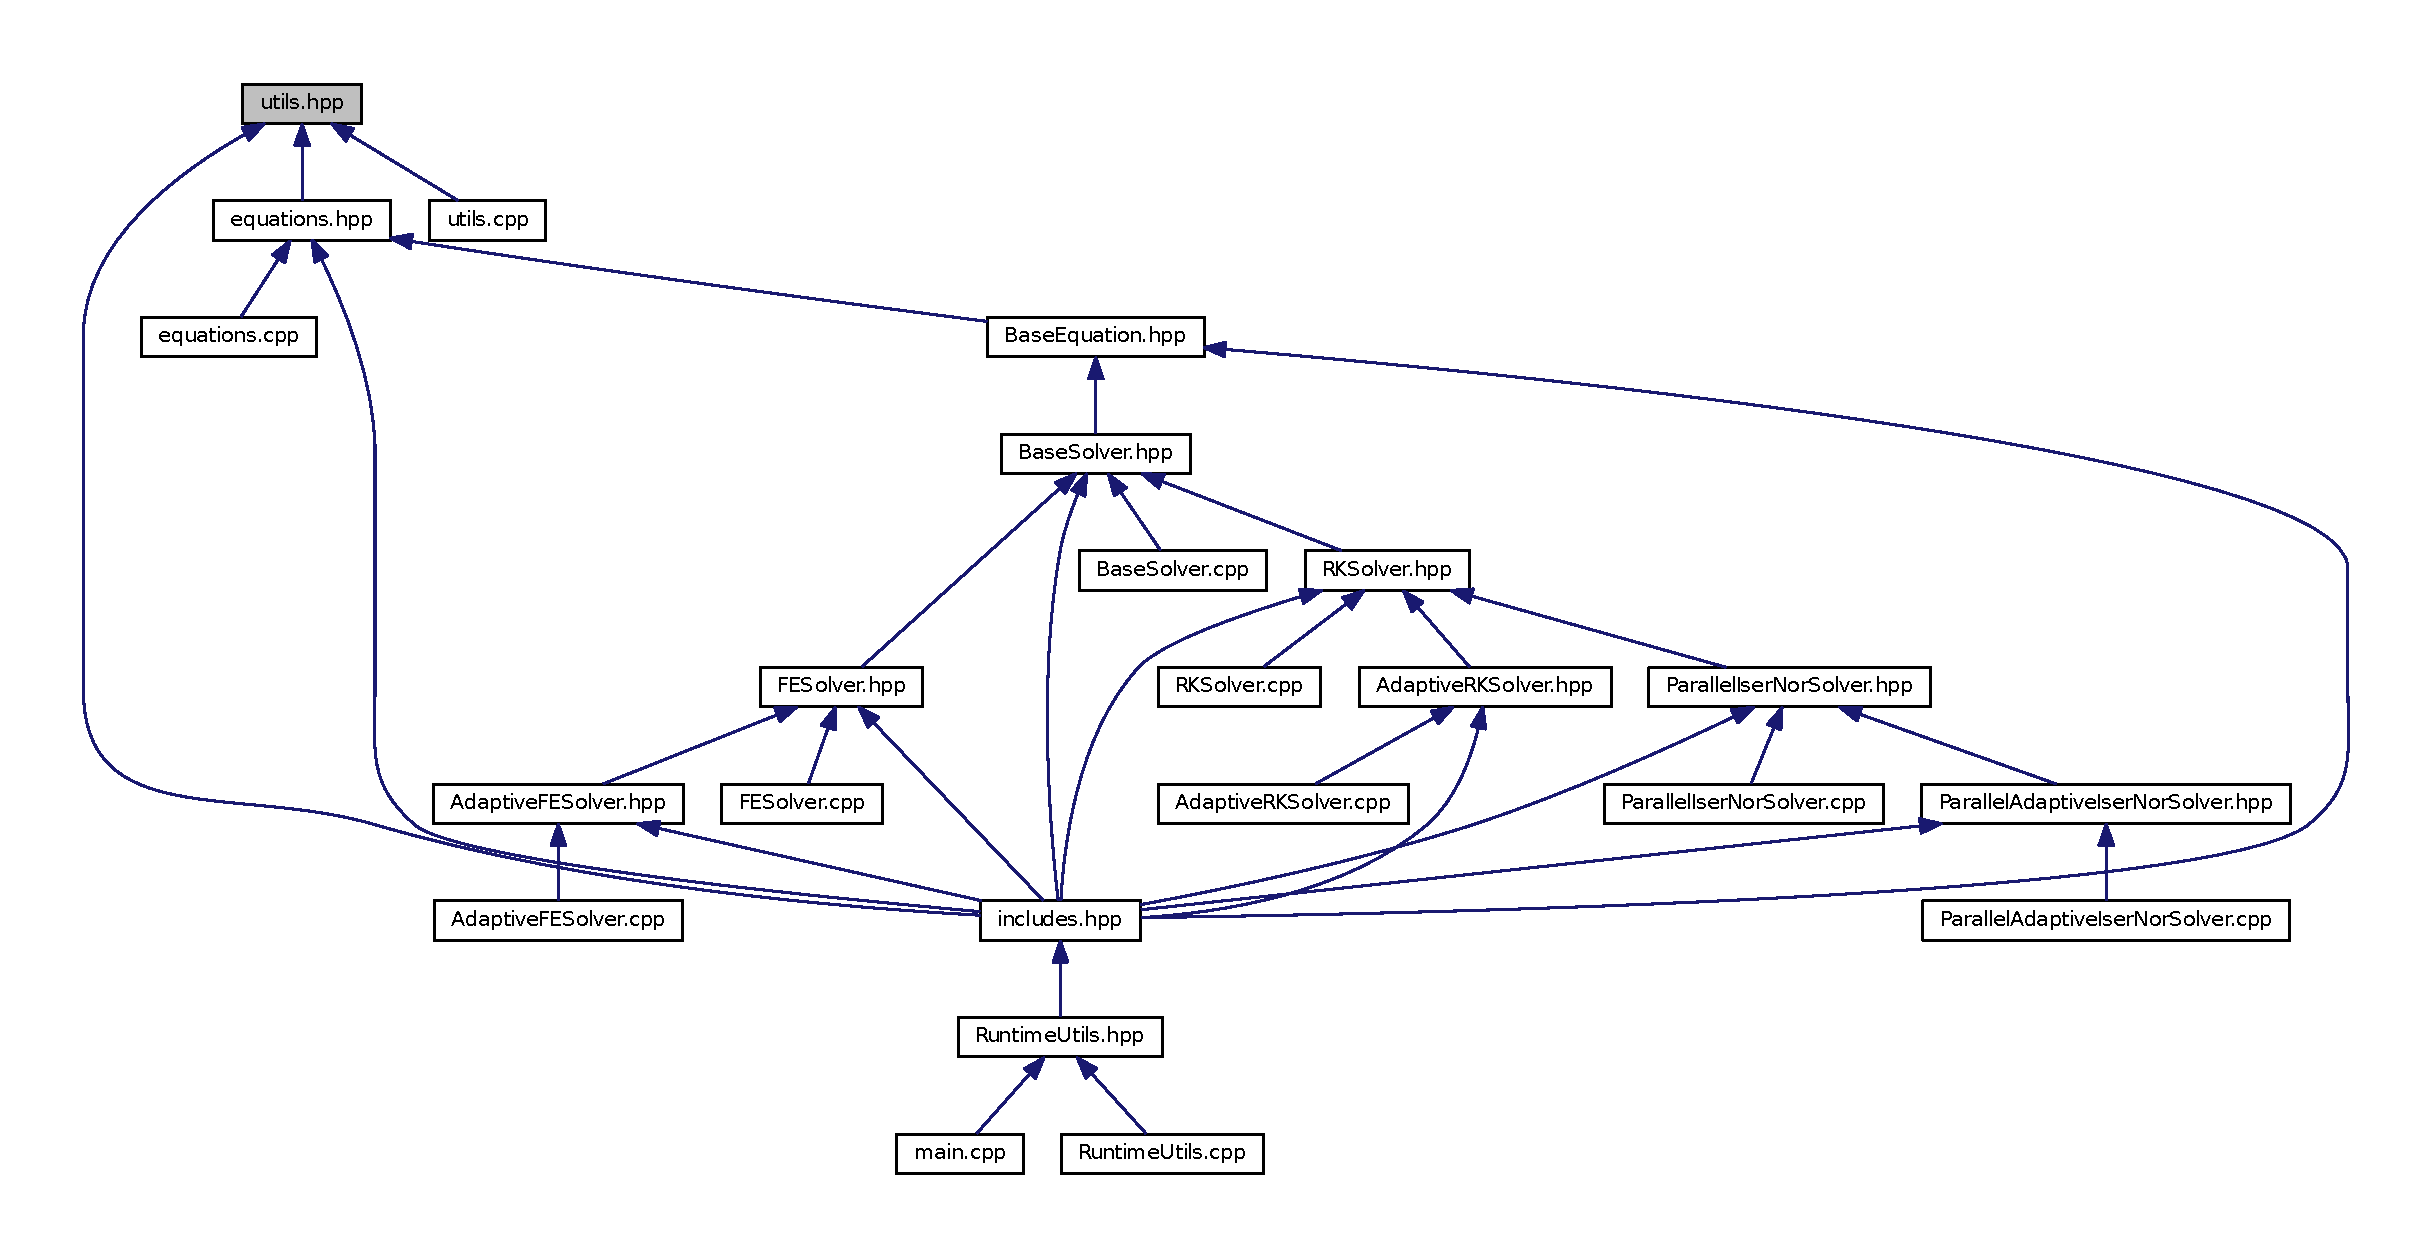
\includegraphics[width=\textwidth]{etc/headers.pdf}
\end{frame}


\begin{frame} %#16
	\frametitle{Implementation choices}
	\begin{itemize}
		\item Seven test functions are provided
		\item Separate FE class is much more efficient than RK specialized class:
		% Moreover, the adaptive RK error is computed differently because there
		% are some unknown (in the general case) quantities that need to be
		% estimated
		\begin{center}
			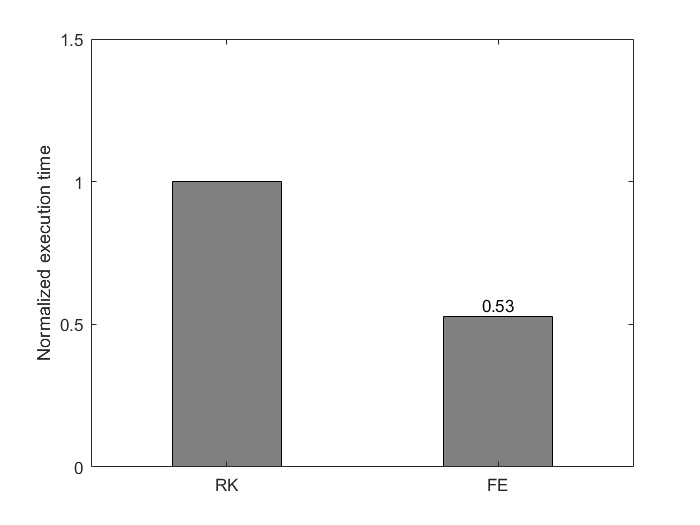
\includegraphics[scale=0.3]{etc/FE_vs_RK.jpeg}
		\end{center}	
		\item Adaptive \texttt{single\_step()} class methods are not efficient
	\end{itemize}
\end{frame}


\begin{frame} %#17
	\frametitle{Parallel Iserles-Nørsett}
	\begin{itemize}
		\item Exploits block-diagonal structure of Butcher array
		\item Runs in parallel on 2 processors, each dealing with one indpendent 2-by-2 block
		\item Fixed point algorithm was used for nonlinear equations
	\end{itemize}
\end{frame}


\begin{frame}[c] %#18
\begin{center}
	\Huge \color{blue} Results
\end{center}
\end{frame}


\begin{frame} %#19
	\frametitle{Comparison between methods}
	\begin{center}
		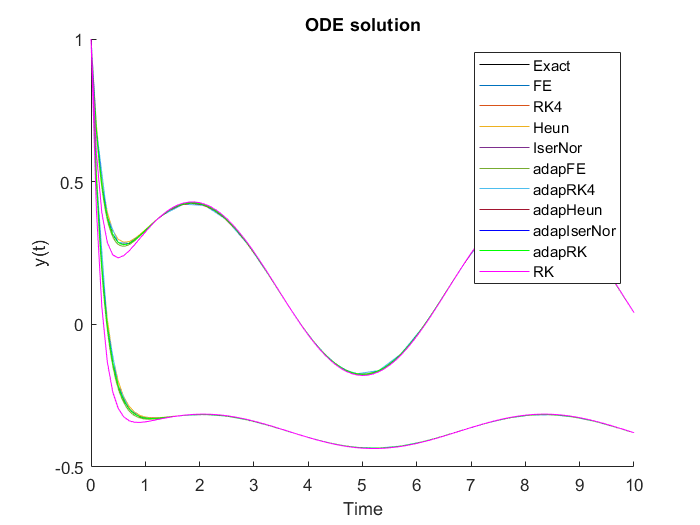
\includegraphics[width=0.8\linewidth]{etc/results_test_4.png} \\
		(components of test \#4)
	\end{center}
\end{frame}


\begin{frame} %#20
	\frametitle{Trend of step in adaptive methods}
	\begin{center}
		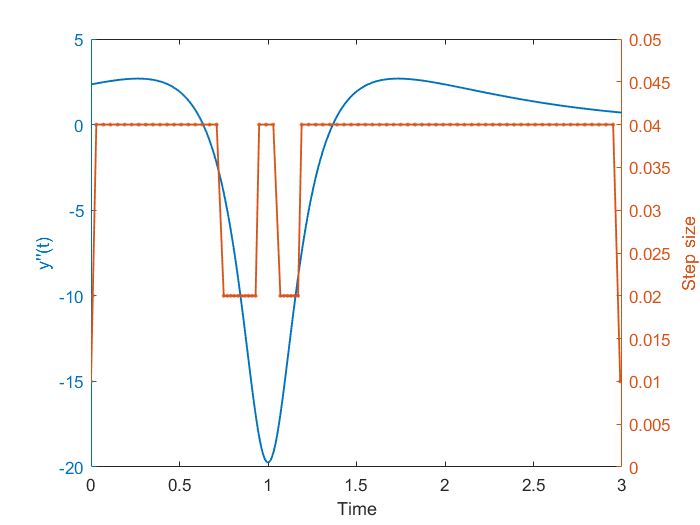
\includegraphics[width=0.8\linewidth]{etc/step_history_7_adapHeun.png} \\
		(test \#7, adaptive Heun method)
	\end{center}	
\end{frame}


\begin{frame} %#21
	\frametitle{Actual efficiency of parallelism}
	Speedup is heavily dependent on the problem function:
	\begin{figure}
		\begin{subfigure}{.5\textwidth}
			\subcaption*{Test \#5}
			\subcaption*{$f(t,y(t)) = -16 y(t)$}
			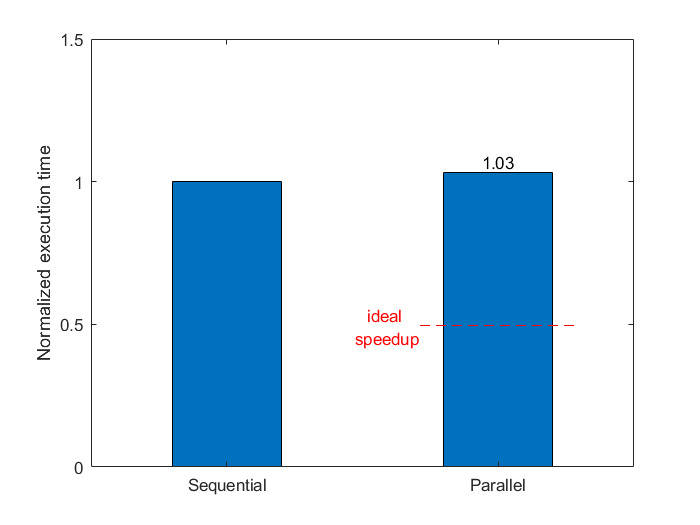
\includegraphics[width=\linewidth]{etc/test5_2.jpeg}
		\end{subfigure}%
		\begin{subfigure}{.5\textwidth}
			\subcaption*{Test \#6}
			\subcaption*{$f(t,y(t)) = \exp_2( -\frac{y(t)}{4} + 6 + 10t) $}
			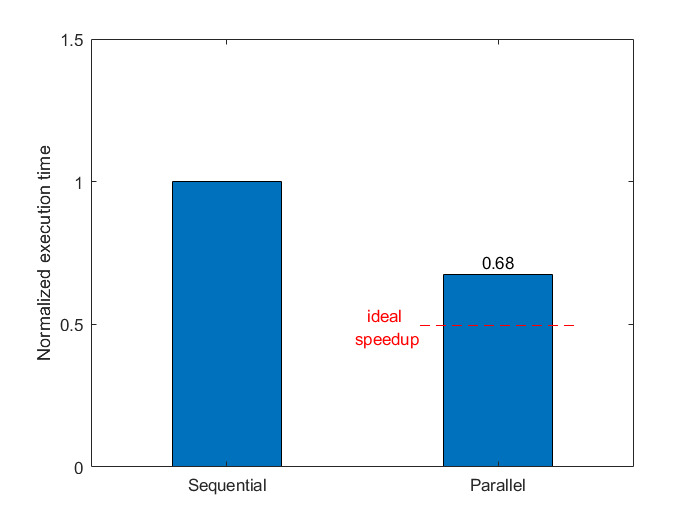
\includegraphics[width=\linewidth]{etc/test6_2.jpeg}
		\end{subfigure}%
	\end{figure}
\end{frame}


\begin{frame} %#22
	\frametitle{Multiple run results}
	\begin{figure}
		\begin{subfigure}{.5\textwidth}
			\subcaption*{Test \#5}
			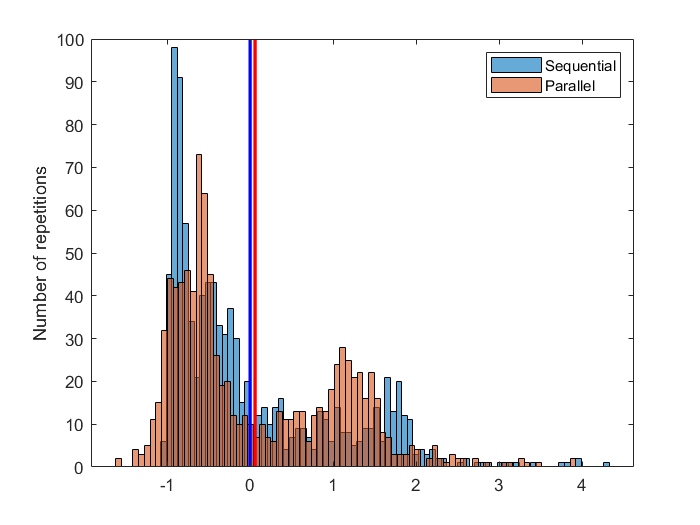
\includegraphics[width=\linewidth]{etc/test5_3.jpeg}
		\end{subfigure}%
		\begin{subfigure}{.5\textwidth}
			\subcaption*{Test \#6}
			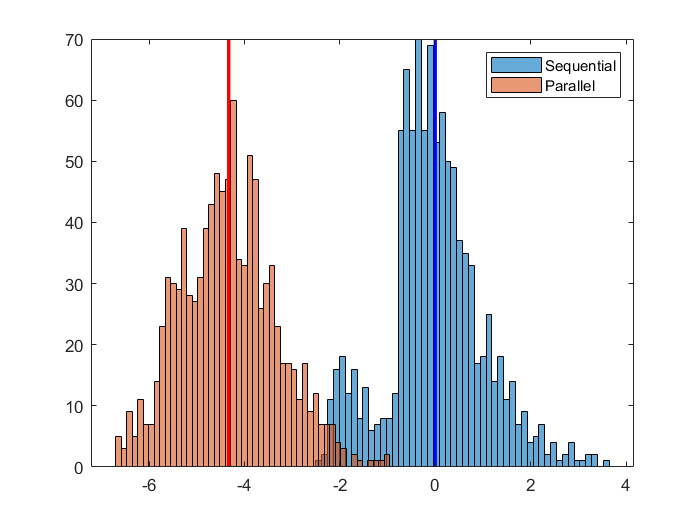
\includegraphics[width=\linewidth]{etc/test6_3.jpeg}
		\end{subfigure}
	\end{figure}
	\begin{center}
		\vspace{16pt}
		Why?
	\end{center}
\end{frame}


\begin{frame} %#23
	\frametitle{Workload distribution}
	\begin{figure}
		\begin{subfigure}{.5\textwidth}
			\subcaption*{Test \#5}
			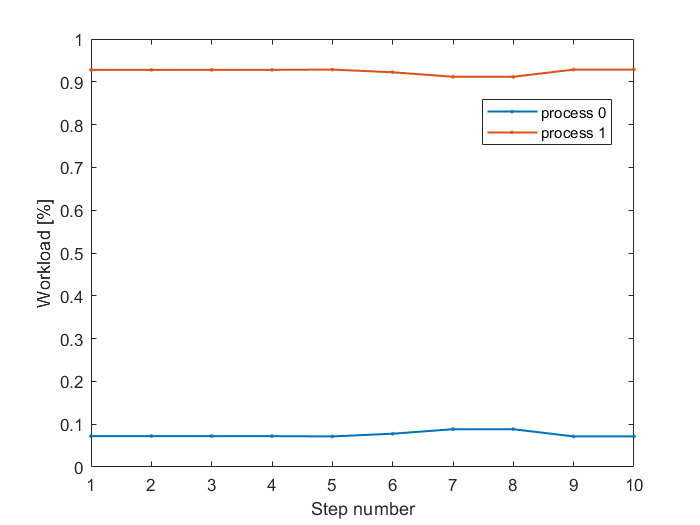
\includegraphics[width=\linewidth]{etc/test5_1.jpeg}
		\end{subfigure}%
		\begin{subfigure}{.5\textwidth}
			\subcaption*{Test \#6}
			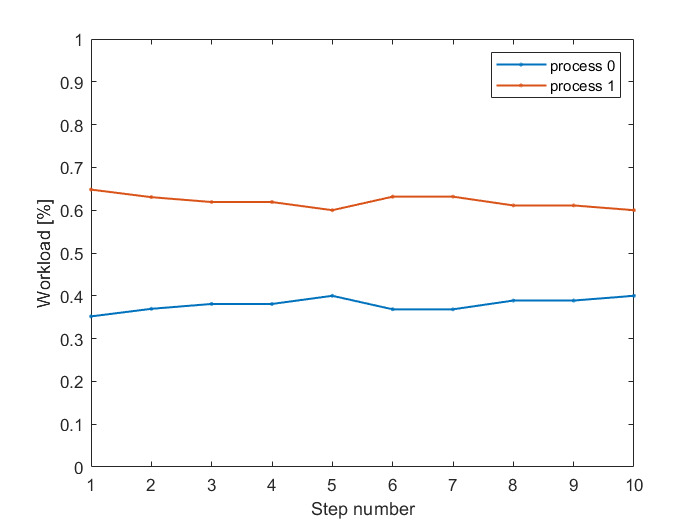
\includegraphics[width=\linewidth]{etc/test6_1.jpeg}
		\end{subfigure}
	\end{figure}
\begin{center}
	\vspace{16pt}
	$\implies$ \textbf{load imbalance}
\end{center}
\end{frame}


\begin{frame} %#24
	\frametitle{A vectorial example}
	\begin{itemize}
		\item Efficiency still depends on the function
		\item Here fixed point iterations are well-balanced among processors:
		% similarly to test 6
	\end{itemize}	
	\begin{center}
		Test \#4: \quad
		$\boldsymbol f(t,\yy(t)) =
		\left[\begin{smallmatrix} -3 & -1 \\ 1 & -5 \end{smallmatrix}\right]
		\yy(t) +
		\left[\begin{smallmatrix} \sin(t) \\ -2t \end{smallmatrix}\right]$
	\end{center}
	\begin{figure}
		\begin{subfigure}{.5\textwidth}
			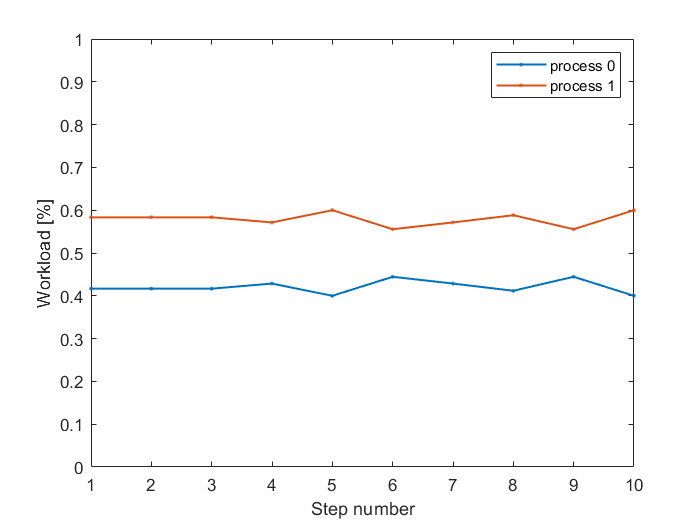
\includegraphics[width=\linewidth]{etc/test4_1.jpeg}
		\end{subfigure}%
		\begin{subfigure}{.5\textwidth}
			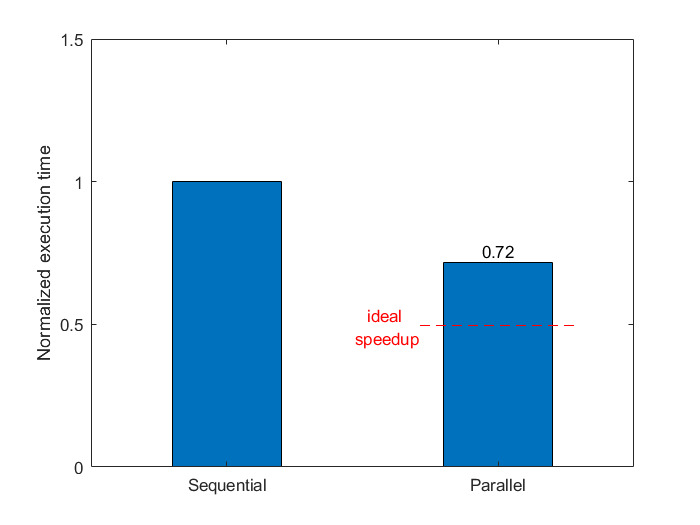
\includegraphics[width=\linewidth]{etc/test4_2.jpeg}
		\end{subfigure}
	\end{figure}
\end{frame}


\begin{frame} %#last
	\frametitle{Bibliography}
	\begin{thebibliography}{9}
		\setbeamertemplate{bibliography item}[book] % or [online] or [article]
		\bibitem{P} Podhaisky, \textit{Parallel two-step Runge-Kutta methods}
		\bibitem{QS} Quarteroni, Saleri, \textit{Calcolo scientifico}
		\bibitem{QSSG} Quarteroni, Sacco, Saleri, Gervasio, \textit{Matematica numerica}
		\bibitem{SI} Solodushkin, Iumanova, \textit{Parallel Numerical Methods for Ordinary Differential Equations: a Survey}	
	\end{thebibliography}
\end{frame}

\end{document}
%%%%%%%%%%%%%%%%%%%%%%%%%%%%%%%%%%%%%%%%%%%%%%%%%%%%%%%%%%%%%%%%%%%%%%%%%%%%%%%%

\begin{frame}
	\frametitle{Title}
	\begin{itemize}
		\item Text
	\end{itemize}
\end{frame}
